\documentclass[tikz]{standalone}

\begin{document}

\tikzset{every picture/.style={line width=0.75pt}} %set default line width to 0.75pt        

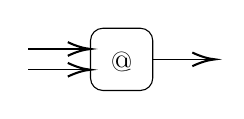
\begin{tikzpicture}[x=0.75pt,y=0.75pt,yscale=-1,xscale=1]
  %uncomment if require: \path (0,300); %set diagram left start at 0, and has height of 300

  %Straight Lines [id:da24815792321220487] 
  \draw    (75,30) -- (103,30) ;
  \draw [shift={(105,30)}, rotate = 180] [color={rgb, 255:red, 0; green, 0; blue, 0 }	][line width=0.75]    (10.93,-3.29) .. controls (6.95,-1.4) and (3.31,-0.3) .. (0,0) .. controls (3.31,0.3) and (6.95,1.4)
  .. (10.93,3.29)   ;
  %Rounded Rect [id:dp6242927445486988] 
  \draw   (45,21) .. controls (45,17.69) and (47.69,15) .. (51,15) -- (69,15) .. controls (72.31,15) and
  (75,17.69) .. (75,21) -- (75,39) .. controls (75,42.31) and (72.31,45) .. (69,45) -- (51,45) .. controls
  (47.69,45) and (45,42.31) .. (45,39) -- cycle ;
  %Straight Lines [id:da40267238619714774] 
  \draw    (15,35) -- (43,35) ;
  \draw [shift={(45,35)}, rotate = 180] [color={rgb, 255:red, 0; green, 0; blue, 0 }	][line width=0.75]    (10.93,-3.29) .. controls (6.95,-1.4) and (3.31,-0.3) .. (0,0) .. controls (3.31,0.3) and (6.95,1.4)
  .. (10.93,3.29)   ;
  %Straight Lines [id:da009042706123695066] 
  \draw    (15,25) -- (43,25) ;
  \draw [shift={(45,25)}, rotate = 180] [color={rgb, 255:red, 0; green, 0; blue, 0 }	][line width=0.75]    (10.93,-3.29) .. controls (6.95,-1.4) and (3.31,-0.3) .. (0,0) .. controls (3.31,0.3) and (6.95,1.4)
  .. (10.93,3.29)   ;

  % Text Node
  \draw (60,31) node   [align=left] {$\displaystyle @$};

\end{tikzpicture}
\end{document}
